% =========================================================================
% METHODOLOGY SECTION / STANDALONE IEEE DRAFT
% Physics-Guided, Identifiability-Aware Extraction of Stanford RRAM Compact-
% Model Parameters from Experimental TaOx I-V Characteristics
%
% This file is intentionally self-contained.  To merge into a full IEEEtran
% manuscript, copy the preamble packages you need and the material from
% \section{Methodology} onward into the main paper.
%
% The method described here is tied to the released pipeline:
%   01_extract_clean_cycles.py
%   02_select_device_representative_curve.py
%   02b_build_cycle_ensemble.py
%   02c_classify_conduction_regimes.py
%   stanford_fit/matlab/*.m
%   04_publication_summary.py, 05_run_ablation.py, 06_run_variability.py,
%   07_run_final.py
% =========================================================================
\documentclass[journal]{IEEEtran}

\usepackage{amsmath,amssymb,amsfonts}
\usepackage{graphicx}
\usepackage{booktabs}
\usepackage{multirow}
\usepackage{siunitx}
\usepackage[ruled,linesnumbered]{algorithm2e}
\usepackage{tikz}
\usetikzlibrary{shapes.geometric,arrows.meta,positioning,fit,calc}

\tikzset{
  stage/.style={rectangle, rounded corners=2pt, draw=black, thick,
    minimum width=5.75cm, minimum height=0.86cm, align=center,
    font=\footnotesize, fill=gray!8},
  datafile/.style={trapezium, trapezium left angle=70, trapezium right angle=110,
    draw=black, minimum height=0.62cm, align=center, font=\scriptsize,
    fill=blue!6, inner xsep=2pt},
  decision/.style={diamond, aspect=2.4, draw=black, thick, align=center,
    font=\scriptsize, fill=orange!10, inner sep=1pt},
  sideout/.style={rectangle, draw=black, dashed, align=center,
    font=\scriptsize, fill=green!6, minimum height=0.62cm},
  arrow/.style={-{Stealth[length=2.4mm]}, thick},
  dasharrow/.style={-{Stealth[length=2.4mm]}, thick, dashed},
}

\begin{document}

\title{Physics-Guided, Identifiability-Aware Extraction of Stanford RRAM
Compact-Model Parameters from Experimental TaO$_x$ Devices}

\author{...}
\maketitle

\begin{abstract}
This paper presents a reproducible extraction flow for fitting the
Stanford--PKU resistive random-access memory (RRAM) compact model to measured
TaO$_x$ DC switching data.  The method is designed for a practical problem
that is often hidden in compact-model calibration: a visually good
$I$--$V$ fit does not by itself prove that the fitted parameters are unique,
physically meaningful, or identifiable from DC data.  The proposed flow first
extracts quality-controlled switching cycles from Keysight B1500 CSV exports
and selects a measured medoid cycle as the nominal fitting target.  It then
classifies the dominant conduction mechanism in each resistance-state segment
using ohmic, Poole--Frenkel, Schottky, and Fowler--Nordheim linearizations
with Bayesian information criterion and a dynamic-permittivity admissibility
test.  The resulting regime map conditions the prior-extraction windows and
the loss weights used during HSPICE-in-the-loop Bayesian optimization.  After
local refinement, the fitted parameter vector is accompanied by an operational
identifiability report based on Fisher/Cramer--Rao analysis at the fitted
optimum and fixed-nuisance one-dimensional loss profiles.  A separate
cluster-bootstrap stage over whole cycles propagates cycle-to-cycle
variability into empirical confidence intervals.  The result is not only a
Stanford-model parameter set, but also a defensible statement of which
parameters are supported by the measured TaO$_x$ data and which are
prior-dominated.
\end{abstract}

% =========================================================================
\section{Methodology}
% =========================================================================

\subsection{Study Design}
\label{sec:study-design}

The objective of this work is to extract Stanford--PKU RRAM compact-model
parameters from measured TaO$_x$ devices in a way that is reproducible,
physics-aware, and honest about parameter uncertainty.  The central claim is
therefore deliberately narrower than ``we can fit an $I$--$V$ curve.''  The
pipeline asks which model parameters are constrained by the available DC
switching measurements, which parameters are only weakly constrained, and
which parameters should not be interpreted as extracted material/device
properties.

Three design choices follow from this objective.

First, conduction physics is treated as a front-end diagnostic rather than an
after-the-fact explanation.  TaO$_x$ RRAM conduction can change with voltage
window, resistance state, cycle, and deposition condition.  The code therefore
classifies each representative curve into ohmic, Poole--Frenkel (PF),
Schottky, Fowler--Nordheim (FN), or unclassified windows before compact-model
fitting.  The classification is used only where the Stanford model can
reasonably respond: ohmic/PF-like bulk regions receive full fitting weight,
whereas Schottky/FN regions, which are not explicitly represented by the
released Stanford current law, are down-weighted but not removed.

Second, a single measured cycle is used for the nominal point estimate.  The
representative curve is a medoid cycle selected from the experimental ensemble,
not a synthetic pointwise median.  This preserves the measured hysteresis
ordering, switching kinks, and compliance-limited portions of the sweep.  The
cycle ensemble is kept separately and is used later for variability and
bootstrap uncertainty.

Third, identifiability is reported as a primary output.  The pipeline produces
a best-fit parameter vector, but it also reports Fisher relative uncertainty,
profile/loss curvature, and bootstrap spread.  Parameters classified as
non-identifiable are retained in the model vector for reproducibility, but
they are not interpreted as independently extracted from DC data.  A two-pass
workflow can optionally freeze such parameters at their prior values and refit
the remaining active subset.

Fig.~\ref{fig:flowchart} summarizes the complete implementation, and
Algorithms~\ref{alg:regimes} and \ref{alg:fit} give the two core procedures.

% -------------------------------------------------------------------------
\subsection{Devices, Conditions, and Measurements}
\label{sec:devices}

The experimental input consists of bipolar DC switching measurements from
TaO$_x$ RRAM devices organized into twelve sample/condition folders
(\texttt{S1}--\texttt{S12}).  The repository includes the deposition-condition
table \texttt{Depos\_Condition.csv}, which records the oxygen percentage and
sputter power associated with each sample folder.  The devices are treated in
the pipeline as measured TaO$_x$ cross-point RRAM cells, consistent with the
TaO$_x$ fabrication and switching studies reported in
\cite{chowdhury2025mwscas,moazzeni2023}.

The raw electrical measurements are Keysight B1500-style CSV exports.  Each
file may contain one or more analysis blocks, and each block contains voltage
and current samples for a SET, RESET, mixed, or otherwise unlabeled sweep.  The
pipeline does not assume that every file is usable.  It first parses all
available measurement blocks, infers branch polarity, assigns a cycle number
within each \texttt{(condition, device)} group, and rejects cycles that do not
contain sufficient information for compact-model fitting.

The Stanford fits use the current compliance value configured for the final
TaO-Fit runs, $I_{\mathrm{cc}}=\SI{5e-4}{\ampere}$.  This value is a
measurement-condition parameter rather than a fitted material parameter: the
Stanford Verilog-A model does not include an instrument compliance circuit, so
the simulated current is clamped to this magnitude after each transient
simulation.

% -------------------------------------------------------------------------
\subsection{Stage 0: Raw Data Extraction and Quality Control}
\label{sec:stage0}

Raw data extraction is performed by \texttt{01\_extract\_clean\_cycles.py}.
The parser reads each CSV using tolerant text handling, detects B1500 analysis
titles, extracts finite voltage-current pairs from \texttt{DataValue} rows,
and falls back to treating the full file as one block if no title rows are
available.  The branch label is inferred from the block title first:
\texttt{reset} gives RESET and \texttt{set} gives SET.  If the title is
uninformative, the code compares the positive and negative voltage extrema to
infer SET, RESET, MIXED, or UNKNOWN.

Each parsed file becomes one cycle record.  A cycle is retained only if all
configured quality criteria are satisfied:
\begin{itemize}
  \item at least 40 finite voltage-current points;
  \item voltage span of at least \SI{1.0}{\volt};
  \item peak absolute current between \SI{1e-9}{\ampere} and
        \SI{1}{\ampere};
  \item median absolute current above the numerical current floor
        \SI{1e-13}{\ampere};
  \item dynamic current range of at least 0.5 decades, computed from the
        5th and 95th percentiles of $|I|$ above the current floor;
  \item both SET and RESET content, unless the command-line option disables
        this requirement.
\end{itemize}

These screens remove shorted devices, open devices, incomplete sweeps,
noise-floor traces, and files with insufficient switching contrast.  The
outputs are (i) \texttt{01\_extracted\_points.csv}, a normalized point table;
(ii) \texttt{01\_cycle\_summary.csv}, a per-cycle quality table; and
(iii) \texttt{01\_device\_summary.csv}, a per-device summary containing the
number of total cycles, number of good cycles, mean quality score, and good
cycle fraction.

% -------------------------------------------------------------------------
\subsection{Stage 1: Representative Device, Programming Segment, and Medoid Cycle}
\label{sec:stage1}

The representative fitting target is produced by
\texttt{02\_select\_device\_representative\_curve.py}.  Unless the user
manually specifies a condition and device, the selected device is the device
with at least five good cycles and the best ranking by three ordered criteria:
number of good cycles, mean quality score, and good-cycle fraction.  If no
device reaches the five-cycle threshold, all devices remain eligible and the
same ranking is applied.  This rule prevents the nominal fitting target from
being chosen by visual preference alone.

For each good cycle and branch, the script then isolates the programming
segment.  Points are sorted by the instrument point index, and the voltage
trace is split when the voltage direction changes.  Candidate segments must
contain at least 20 points and span at least \SI{0.3}{\volt}.  SET candidates
are scored for positive polarity and positive-going voltage; RESET candidates
are scored for negative polarity and negative-going voltage.  The
highest-scoring segment is retained as the programming segment for that
cycle/branch.

The default representative mode is \texttt{medoid-cycle}.  For each branch, all
programming cycles are interpolated in $\log_{10}|I|$ onto a common voltage
grid.  The branch-typical behavior is the median log-current at each grid
voltage.  The score of cycle $c$ on branch $b$ is
\begin{equation}
  s_{c,b} =
  \operatorname{median}_{v}\left|
  \log_{10}|I_{c,b}(v)| -
  \operatorname{median}_{c'}\log_{10}|I_{c',b}(v)|
  \right|,
  \label{eq:medoid-score}
\end{equation}
computed only where enough cycles overlap.  The script ranks cycles within
each branch, converts the ranks to rank fractions, and chooses one real cycle
that minimizes the mean branch rank fraction across the available SET and
RESET branches.  If no single cycle covers both branches adequately, the code
falls back to the best measured cycle per branch.  The output file keeps the
downstream median-column schema, but in \texttt{medoid-cycle} mode these
values are the measured values of the selected cycle.  Consequently, the
nominal point-estimate fit is anchored to an experimentally observed sweep,
not to a synthetic average.

The separate script \texttt{02b\_build\_cycle\_ensemble.py} builds a long-form
ensemble table for the same selected device.  This table contains every good
cycle, tagged by \texttt{representative\_cycle\_id} and point index.  The
ensemble is not used to change the nominal point estimate in Stages 1--4; it
is used in Stage 7 for leave-one-cycle-out and cluster-bootstrap analyses.

% -------------------------------------------------------------------------
\subsection{Stage 2: Conduction-Regime Classification}
\label{sec:regimes}

Stage 2 automates the conduction-mechanism analysis used in the experimental
TaO$_x$ study
\cite{chowdhury2025mwscas}.  It produces a regime map that is later consumed
by the prior extractor and the loss function.

\subsubsection{State segmentation}
The representative butterfly cycle is sorted by the sequence index and split
by branch.  The SET branch is divided at its maximum voltage into
\texttt{SET\_HRS\_PRE} and \texttt{SET\_LRS\_POST}; the RESET branch is divided
at its minimum voltage into \texttt{RESET\_LRS\_PRE} and
\texttt{RESET\_HRS\_POST}.  This sequence-based split is important because
forward and return sweeps may occupy overlapping voltage ranges while
corresponding to different resistance states.

\subsubsection{Candidate transport mechanisms}
Within each state segment, the code converts voltage and current to
$V=|V_{\mathrm{meas}}|$ and $I=|I_{\mathrm{meas}}|$, removes points with
$V<\SI{0.05}{\volt}$ or $I<\SI{1e-13}{\ampere}$, and removes the apparent
compliance plateau by discarding points with
$I\ge 0.95\max(I)$ in that cleaned segment.  Sliding windows of length
\[
  w=\max(8,\lceil N/3\rceil)
\]
are evaluated with stride $\lfloor w/4\rfloor$.  On each window, four standard
linearized regressions are tested:
\begin{align}
  \text{ohmic:} &&
  \ln I &= m\ln V + b, &
  0.8 \le m \le 1.2, \label{eq:ohmic}\\
  \text{PF:} &&
  \ln(I/V) &= s_{\mathrm{PF}}\sqrt{V}+b, &
  s_{\mathrm{PF}}>0, \label{eq:pf}\\
  \text{Schottky:} &&
  \ln I &= s_{\mathrm{S}}\sqrt{V}+b, &
  s_{\mathrm{S}}>0, \label{eq:schottky}\\
  \text{FN:} &&
  \ln(I/V^2) &= s_{\mathrm{FN}}/V+b, &
  s_{\mathrm{FN}}<0. \label{eq:fn}
\end{align}

PF and Schottky linearizations are nearly collinear on short voltage windows.
The classifier therefore applies a physical admissibility test before
comparing regression scores.  For a fitted square-root-voltage slope $s$, the
dynamic relative permittivity implied by the PF or Schottky expression is
\begin{equation}
  \varepsilon_r^{\mathrm{dyn}}
  =
  \frac{q^3}{\pi\varepsilon_0 t_{\mathrm{ox}}(s kT)^2}
  \begin{cases}
    1, & \mathrm{PF},\\
    1/4, & \mathrm{Schottky}.
  \end{cases}
  \label{eq:eps-dyn}
\end{equation}
The candidate is admitted only if
$\varepsilon_r^{\mathrm{dyn}}\in[1,60]$ under the configured
$t_{\mathrm{ox}}=\SI{7}{\nano\meter}$ and $T=\SI{300}{\kelvin}$.  This broad
range is intentionally conservative; it prevents an arbitrary
square-root-voltage trend from being labeled PF or Schottky while still
allowing realistic TaO$_x$ dielectric variation.

For all admitted candidates, model selection uses the Bayesian information
criterion
\begin{equation}
  \mathrm{BIC}
  = n\ln\left(\frac{\mathrm{RSS}}{n}\right)+2\ln n,
  \label{eq:bic}
\end{equation}
where each linearized fit has two fitted coefficients.  The lowest-BIC
admissible mechanism wins.  Windows for which no candidate passes the
sign/range and permittivity checks are labeled \texttt{unclassified}.
Consecutive windows with the same label are merged, and the winning
linearization is refit over the merged voltage span to report the final slope,
intercept, $R^2$, BIC, dynamic permittivity, and point count.

\subsubsection{Regime-map outputs}
The regime map contains the columns
\texttt{branch}, \texttt{state}, \texttt{v\_lo}, \texttt{v\_hi},
\texttt{mechanism}, \texttt{slope}, \texttt{intercept}, \texttt{r2},
\texttt{bic}, \texttt{eps\_r\_dyn}, \texttt{n\_points}, and
\texttt{stanford\_valid}.  The last flag is true for ohmic and PF windows and
false for Schottky, FN, and unclassified regions.  When the per-cycle ensemble
is provided, each cycle is also classified at the state-segment level; the
fraction of cycles assigned to each mechanism is reported as a
cycle-to-cycle mechanism-stability metric.

\begin{algorithm}[!t]
\caption{Conduction-regime classification}
\label{alg:regimes}
\footnotesize
\KwIn{Representative curve $D$; optional cycle ensemble $\mathcal{E}$;
$t_{\mathrm{ox}}$, $T$, and admissible
$\varepsilon_r^{\mathrm{dyn}}\in[1,60]$}
\KwOut{Regime map $\mathcal{R}$ and optional mechanism-stability table}
sort $D$ by the butterfly sequence index\;
split SET at maximum voltage and RESET at minimum voltage to obtain
\texttt{SET\_HRS\_PRE}, \texttt{SET\_LRS\_POST},
\texttt{RESET\_LRS\_PRE}, and \texttt{RESET\_HRS\_POST}\;
\ForEach{state segment $S$}{
  convert to $V=|V|$, $I=|I|$; remove low-voltage, current-floor, and
  compliance-plateau points\;
  set $w=\max(8,\lceil |S|/3\rceil)$ and slide by $\lfloor w/4\rfloor$\;
  \ForEach{window $W$}{
    regress Eqs.~(\ref{eq:ohmic})--(\ref{eq:fn})\;
    reject candidates that fail slope constraints or the
    $\varepsilon_r^{\mathrm{dyn}}$ check\;
    assign the admitted mechanism with minimum BIC, or \texttt{unclassified}\;
  }
  merge adjacent same-label windows and refit each merged span\;
  set \texttt{stanford\_valid}=1 for ohmic/PF and 0 otherwise\;
}
\If{$\mathcal{E}$ is provided}{
  classify each cycle by state segment and report mechanism fractions\;
}
\end{algorithm}

% -------------------------------------------------------------------------
\subsection{Stanford Compact Model and HSPICE Forward Map}
\label{sec:model}

The fitted device model is the Stanford--PKU RRAM Verilog-A model
\texttt{rram\_v\_1\_0\_0} \cite{guan2012spice,jiang2014stanford}, simulated
with HSPICE through generated transient netlists.  The model state variable is
the conductive-filament gap $g$.  The terminal current is
\begin{equation}
  I_{\mathrm{tb}}
  = I_0 \exp\left(-\frac{g}{g_0}\right)
    \sinh\left(\frac{V_{\mathrm{tb}}}{V_0}\right),
  \label{eq:stanford-current}
\end{equation}
and the deterministic gap rate implemented in the Verilog-A source is
\begin{equation}
  \frac{dg}{dt}
  =
  -\nu_0
  \exp\left(-\frac{qE_a}{kT_{\mathrm{cur}}}\right)
  \sinh\left(
    \frac{\gamma a_0}{t_{\mathrm{ox}}}
    \frac{qV_{\mathrm{tb}}}{kT_{\mathrm{cur}}}
  \right),
  \label{eq:stanford-gap}
\end{equation}
with
\begin{equation}
  T_{\mathrm{cur}} = T_{\mathrm{ini}} + |V_{\mathrm{tb}}I_{\mathrm{tb}}R_{\mathrm{th}}|.
  \label{eq:temperature}
\end{equation}
The gap is integrated from \texttt{gap\_ini} and clamped to
$[\texttt{gap\_min},\texttt{gap\_max}]$.  The released HSPICE model computes
the field-enhancement factor as
\begin{equation}
  \gamma =
  \gamma_{\mathrm{ini}} -
  \beta\left(\frac{g}{\SI{1}{\nano\meter}}\right)^3,
  \qquad
  \gamma_{\mathrm{ini}} =
  \begin{cases}
    \gamma_0, & V_{\mathrm{tb}}\ge 0,\\
    16, & V_{\mathrm{tb}}<0,
  \end{cases}
  \label{eq:gamma}
\end{equation}
and sets $\gamma=0$ when
$\gamma |V_{\mathrm{tb}}|/t_{\mathrm{ox}}<F_{\min}$.  This negative-bias
override is an important implementation detail: although reset-side
\texttt{gamma0\_res} is retained in the parameter/prior table, the default
optimization does not actively fit it because the Verilog-A branch overrides
$\gamma_0$ under negative bias.

The HSPICE deck places a series resistor $R_s$ between the voltage source and
the RRAM device.  This resistor accounts for probe/parasitic resistance and
softens the LRS branch; it is not a substitute for the SMU compliance.  For
each objective evaluation the code runs two separate transients: one SET
transient, initialized in HRS, and one RESET transient, initialized in LRS.
Polarity-split parameters allow the compact model to fit asymmetric measured
SET and RESET behavior while keeping the scale/parasitic parameters shared.

The measured voltage samples are replayed as a piecewise-linear source.  The
time increment between adjacent samples is
\[
  \Delta t_i =
  \max\left(\frac{|V_i-V_{i-1}|}{\SI{1e5}{\volt\per\second}},\,
  \SI{1e-12}{\second}\right),
\]
and the transient step is configured as \SI{1e-6}{\second}.  This is a
quasi-static mapping chosen for tractable HSPICE simulation; the fitted
$\nu_0$ and $E_a$ absorb the effective sweep-time scale.  The simulated source
current is parsed from the HSPICE \texttt{.lis} or \texttt{.mt0} table,
converted from source-current sign convention to the project device-current
convention, interpolated back to the measured time stamps, and then clamped to
$|I|\le I_{\mathrm{cc}}$.

% -------------------------------------------------------------------------
\subsection{Stage 3: Regime-Conditioned Priors}
\label{sec:priors}

Priors are extracted in \texttt{stage1\_extract\_priors.m}.  Each parameter
receives a mean $\mu$, standard deviation $\sigma$, and hard lower/upper
bounds.  The prior vector contains 21 entries: seven shared parameters,
twelve polarity-split parameters, and two branch-specific initial gaps.  The
default final configuration uses $T=\SI{300}{\kelvin}$,
$t_{\mathrm{ox}}=\SI{7}{\nano\meter}$,
$a_0=\SI{0.25}{\nano\meter}$, and
$\varepsilon_r=25$.

When a regime map is supplied, the prior windows are selected from the
classified physics.  This is the main distinction from a fixed-window
compact-model fit.

\subsubsection{LRS sinh prior for $I_0$ and $V_0$}
The LRS current scale is estimated from the low-voltage ohmic window of
\texttt{SET\_LRS\_POST}.  If no regime map is available, the legacy fallback
window is $0.02\le V\le\SI{0.6}{\volt}$.  The fit uses the SET return half
when possible and excludes the compliance plateau.  The regression model is
\begin{equation}
  I(V) = A\sinh\left(\frac{V}{V_0}\right),
  \label{eq:sinh-prior}
\end{equation}
solved in log-parameter space with Nelder--Mead.  Since the LRS gap is seeded
near $g_{\min}$, the current-scale prior is
\begin{equation}
  \mu_{I_0} = A\exp\left(\frac{g_{\min}}{g_{0,\mathrm{prior}}}\right),
  \label{eq:i0-prior}
\end{equation}
with uncertainty propagated from the residual scale and the $g_0$ prior.  The
implemented lower bound on the $I_0$ prior uncertainty is 25\% of
$|\mu_{I_0}|$.

\subsubsection{PF priors for $\gamma_0$ and $E_a$}
The HRS PF window of \texttt{SET\_HRS\_PRE} is used for the SET-side
\texttt{gamma0\_set}/\texttt{Ea\_set} priors, and the HRS PF window of
\texttt{RESET\_HRS\_POST} is used for the reset-side
\texttt{gamma0\_res}/\texttt{Ea\_res} priors.  For a PF regression
\[
  \ln(I/V) = \kappa\sqrt{V}+b,
\]
the implemented mapping is
\begin{align}
  \mu_{\gamma_0}
  &=
  2\kappa\sqrt{\pi\varepsilon t_{\mathrm{ox}}}
  \frac{kT}{q}\frac{t_{\mathrm{ox}}}{a_0^2},
  \label{eq:gamma-prior}\\
  \mu_{E_a}
  &=
  -b\frac{kT}{q},
  \label{eq:ea-prior}
\end{align}
followed by clipping to the hard bounds in Table~\ref{tab:priors}.  If a
regime map is present but no PF window exists for a branch, the code does not
force a PF fit onto non-PF data.  Instead, it keeps the literature-centered
defaults $\gamma_0=16.5$ and $E_a=\SI{0.6}{\electronvolt}$, inflates their
standard deviations to 12 and 0.4, respectively, and records the missing PF
prior in the \texttt{pf\_available} flag.

\subsubsection{Remaining priors and active set}
The series-resistance mean is estimated from the measured LRS resistance when
available; otherwise the fallback is sized from
$\SI{5}{\volt}/I_{\mathrm{cc}}$ and then clamped to
$[10,10^5]\,\Omega$ before optimization bounds are applied.  The remaining
priors are literature- or structure-centered values with deliberately broad
bounds.

By default, the optimizer varies 16 parameters:
\[
\begin{gathered}
I_0,\; g_0,\; R_s,\; \gamma_{0,\mathrm{set}},\\
V_{0,\mathrm{set}}, V_{0,\mathrm{res}},
E_{a,\mathrm{set}}, E_{a,\mathrm{res}},
F_{\min,\mathrm{set}}, F_{\min,\mathrm{res}},\\
\nu_{0,\mathrm{set}}, \nu_{0,\mathrm{res}},
g_{\max,\mathrm{set}}, g_{\max,\mathrm{res}},
g_{\mathrm{ini,set}}, g_{\mathrm{ini,res}}.
\end{gathered}
\]
The other prior-table parameters, including $\beta$, $R_{\mathrm{th}}$,
$g_{\min}$, $t_{\mathrm{ox}}$, and \texttt{gamma0\_res}, remain fixed at their
prior means unless the user overrides \texttt{active\_params} in the YAML
configuration.

\begin{table*}[!t]
\centering
\caption{Prior table implemented by \texttt{stage1\_extract\_priors.m}.
Values shown in nanometers or V/nm are stored in SI units in the code.}
\label{tab:priors}
\footnotesize
\begin{tabular}{@{}llllll@{}}
\toprule
Parameter & Source & Mean & Std. dev. & Bounds & Unit\\
\midrule
$I_0$ & LRS sinh & Eq.~(\ref{eq:i0-prior}) & $\ge 0.25|\mu|$ & $[10^{-8},9.9{\times}10^{-3}]$ & A\\
$g_0$ & config/lit. & 0.275 & 0.05 & $[0.15,0.50]$ & nm\\
$\beta$ & config/lit. & 1.25 & 0.5 & $[0.1,5]$ & --\\
$R_{\mathrm{th}}$ & config/lit. & $2.1{\times}10^3$ & $10^3$ & $[1,10^6]$ & K/W\\
$g_{\min}$ & structure & 0.10 & 0.05 & $[0.05,1.0]$ & nm\\
$t_{\mathrm{ox}}$ & config & 7.0 & 0.5 & $[2,10]$ & nm\\
$R_s$ & LRS/fallback & $R_{\mathrm{LRS}}$ or $5/I_{\mathrm{cc}}$ & $0.5\mu$ & $[10,10^6]$ & $\Omega$\\
$V_{0,\{\mathrm{set,res}\}}$ & LRS sinh & Eq.~(\ref{eq:sinh-prior}) & fit scale & $[0.05,2.0]$ & V\\
$\gamma_{0,\{\mathrm{set,res}\}}$ & PF or default & Eq.~(\ref{eq:gamma-prior}) or 16.5 & $0.4\mu$ or 12 & $[4,24]$ & --\\
$E_{a,\{\mathrm{set,res}\}}$ & PF or default & Eq.~(\ref{eq:ea-prior}) or 0.6 & 0.25 or 0.4 & $[0.1,0.99]$ & eV\\
$F_{\min,\{\mathrm{set,res}\}}$ & config/lit. & 1.4 & 0.42 & $[0.5,2.99]$ & V/nm\\
$\nu_{0,\{\mathrm{set,res}\}}$ & config/lit. & 10 & 5 & $[0.1,19.9]$ & m/s\\
$g_{\max,\{\mathrm{set,res}\}}$ & structure & 1.7 & 0.3 & $[1,10]$ & nm\\
$g_{\mathrm{ini,set}}$ & HRS seed & 1.4 & 0.3 & $[0.5,2.5]$ & nm\\
$g_{\mathrm{ini,res}}$ & LRS seed & 0.10 & 0.05 & $[0.05,0.5]$ & nm\\
\bottomrule
\end{tabular}
\end{table*}

% -------------------------------------------------------------------------
\subsection{Stage 4: Mechanism-Aware Objective Function}
\label{sec:loss}

The optimizer minimizes a variance-scaled log-current loss plus switching
threshold and prior penalties.  For measured point $i$,
\begin{equation}
  r_i(\boldsymbol{\theta})
  =
  \frac{\log_{10}|I_i^{\mathrm{sim}}(\boldsymbol{\theta})|
  -\log_{10}|I_i^{\mathrm{meas}}|}
  {\sigma_i^{\log I}}.
  \label{eq:residual}
\end{equation}
The noise scale is computed from the current interquartile range when such an
ensemble-derived spread is present:
\begin{equation}
  \sigma_i^{\log I}
  =
  \frac{|q_{75,i}-q_{25,i}|}{1.35\,|I_i^{\mathrm{med}}|\ln 10}.
  \label{eq:sigma-log}
\end{equation}
Non-finite or non-positive values are replaced by 0.2 decades, and all values
are floored at 0.05 decades.  This detail matters for the medoid point
estimate: because the medoid CSV contains a single measured cycle in the
median/q25/q75 schema, $q_{75}=q_{25}$ and the point-estimate fit uses the
0.2-decade fallback.  In the bootstrap stage, the resampled ensemble is
aggregated by branch and point index, so Eq.~(\ref{eq:sigma-log}) reflects
cycle-to-cycle spread.

If mechanism weighting is enabled and a regime map is available, each point is
assigned a weight
\begin{equation}
  w_i =
  \begin{cases}
    1, & \text{ohmic, PF, or no covering classified window},\\
    w_{\mathrm{nb}}, & \text{covered only by Schottky or FN windows},
  \end{cases}
  \label{eq:weights}
\end{equation}
with $w_{\mathrm{nb}}=0.3$ in the final configuration.  The SET and RESET
current losses are weighted mean-squared residuals,
\begin{equation}
  L_b =
  \frac{\sum_{i\in b} w_i r_i^2}{\sum_{i\in b}w_i},
  \qquad b\in\{\mathrm{SET},\mathrm{RESET}\}.
  \label{eq:branch-loss}
\end{equation}
The state assignment for a point is based on its sequence position relative to
the branch voltage extremum, not solely on voltage magnitude, so forward and
return segments remain distinct.

The total objective is
\begin{equation}
  L(\boldsymbol{\theta})
  =
  L_{\mathrm{SET}}+L_{\mathrm{RESET}}
  +0.5L_V+0.1L_{\mathrm{prior}}.
  \label{eq:loss}
\end{equation}
Here $L_V$ penalizes mismatch between measured and simulated switching
thresholds, where the threshold is the voltage of maximum
$d\log_{10}|I|/dV$ for SET and minimum $d\log_{10}|I|/dV$ for RESET.  The
voltage scale is the median measured voltage step, floored at
\SI{0.01}{\volt}.  The prior term is
\[
  L_{\mathrm{prior}}
  =
  \sum_j
  \left(\frac{\theta_j-\mu_j}{\sigma_j}\right)^2
\]
over finite prior standard deviations.  In the \texttt{plain} ablation mode,
the prior standard deviations are set to infinity, removing this prior
penalty and expanding the search to the hard physical bounds.

% -------------------------------------------------------------------------
\subsection{Stage 5: Global Optimization and Local Refinement}
\label{sec:optimization}

Global search is performed by MATLAB \texttt{bayesopt} in
\texttt{stage3\_bayesopt\_driver.m}.  The final configuration uses 48
quasi-random seed evaluations and 160 adaptive evaluations with the
expected-improvement-plus acquisition function, deterministic objective
setting, no parallelism, and random seed 0.  Parameters with strong scale
behavior are optimized with logarithmic transforms where configured.  The
wide-search parameters $I_0$, $g_0$, $R_s$, $\nu_{0,\mathrm{set}}$,
$\nu_{0,\mathrm{res}}$, $F_{\min,\mathrm{set}}$, and
$F_{\min,\mathrm{res}}$ use their full hard bounds.  Other active parameters
use $[\mu_j-3\sigma_j,\mu_j+3\sigma_j]$ clipped to the hard bounds, unless the
plain-prior ablation expands them to the full bounds.

The Bayesian-optimization result is refined by \texttt{stage4\_local\_refine.m}
using Nelder--Mead \texttt{fminsearch} in log-parameter coordinates.  The
default local-refinement budget is 100 function evaluations.  Any proposal
outside the hard bounds receives a large penalty, preserving positivity and
physical bounds without requiring constrained-simplex machinery.  A nominal
point-estimate run therefore costs
$2(48+160+100)=616$ HSPICE branch transients, because each objective
evaluation requires one SET and one RESET simulation.

% -------------------------------------------------------------------------
\subsection{Stage 6: Operational Identifiability}
\label{sec:identifiability}

Identifiability is evaluated after optimization at the fitted optimum
$\hat{\boldsymbol{\theta}}$.  This ordering is intentional: the Fisher
information and the local sensitivity directions are properties of the fitted
solution, not of the prior mean.  The code writes a per-condition
\texttt{identifiability\_report.csv} containing the parameter value, active
flag, Fisher relative uncertainty, Fisher class, profile verdict, and PF-prior
availability.

\subsubsection{Fisher/Cramer--Rao analysis}
The finite-difference sensitivity matrix is computed for every parameter in
the prior vector, not only for the active subset.  For parameter $\theta_j$,
the code perturbs the fitted optimum with a relative step of $10^{-3}$,
clips the lower perturbation at the lower bound, and forms the log-parameter
sensitivity
\begin{equation}
  S_{ij}
  =
  \frac{
  \log_{10}|I_i(\theta_j^+)|
  -\log_{10}|I_i(\theta_j^-)|}
  {\ln\theta_j^+ - \ln\theta_j^-}.
  \label{eq:sensitivity}
\end{equation}
After variance scaling, the Fisher matrix is
\begin{equation}
  F = \widetilde S^{\mathsf T}\widetilde S.
  \label{eq:fisher}
\end{equation}
Because compact-model parameterizations are often sloppy, $F$ may be
rank-deficient.  The effective standard deviation is therefore computed from
the pseudo-inverse,
\[
  \sigma_j^{\mathrm{eff}} = \sqrt{[F^+]_{jj}},
\]
and the relative uncertainty is
\[
  \rho_j =
  \frac{\sigma_j^{\mathrm{eff}}}{|\hat{\theta}_j|}.
\]
The implemented classification is:
\[
\begin{cases}
\rho_j < 0.5, & \text{identifiable},\\
0.5 \le \rho_j < 2, & \text{weakly identifiable},\\
\rho_j \ge 2, & \text{non-identifiable}.
\end{cases}
\]
The eigenspectrum and eigenvectors of $F$ are also archived to expose
near-null parameter combinations that are not visible from scalar uncertainty
alone.

\subsubsection{Fixed-nuisance loss profiles}
Fisher analysis is local and linearized, so the final configuration also runs
a one-dimensional loss-profile stage for active parameters.  For each active
parameter, \texttt{stage4b\_profile\_likelihood.m} evaluates the objective at
seven grid points across
\[
  [\max(l_j,\hat{\theta}_j-2\sigma_j),\,
    \min(u_j,\hat{\theta}_j+2\sigma_j)]
\]
with all other parameters held fixed at the fitted optimum.  This is a
fixed-nuisance profile scan rather than a full nuisance-parameter reoptimization,
chosen to make the check feasible with HSPICE-in-the-loop simulation.  Let
$\Delta_{\mathrm{lo}}$ and $\Delta_{\mathrm{hi}}$ be the loss increases at the
two scan edges relative to the optimum, and let
$\Delta=\min(\Delta_{\mathrm{lo}},\Delta_{\mathrm{hi}})$.  The implemented
verdict is \texttt{flat\_non\_identifiable} for $\Delta<1$,
\texttt{weakly\_identifiable} for $1\le\Delta<4$, and
\texttt{identifiable} for $\Delta\ge4$.

\subsubsection{Interpretation policy}
The reported fitted vector remains the actual vector used in simulation, even
when some entries are weak or non-identifiable.  The manuscript interpretation
is stricter: identifiable parameters may be discussed as data-supported
extractions; weakly identifiable parameters should be discussed with caution;
non-identifiable parameters should be described as prior-dominated under the
available DC data.  If desired, the two-pass \texttt{auto\_active} workflow
uses a previous \texttt{identifiability\_report.csv} to freeze
non-identifiable parameters and refit the remaining active subset.

% -------------------------------------------------------------------------
\subsection{Stage 7: Validation and Cycle-to-Cycle Uncertainty}
\label{sec:uncertainty}

Validation is performed in \texttt{stage5\_validate.m}.  For the final fitted
vector, the code simulates the SET and RESET branches, computes unweighted
log-current residuals in decades, and reports branch-wise RMSE together with
the Durbin--Watson statistic:
\begin{equation}
  \mathrm{DW} =
  \frac{\sum_{i=2}^{n}(e_i-e_{i-1})^2}{\sum_{i=1}^{n}e_i^2}.
  \label{eq:dw}
\end{equation}
The RMSE measures magnitude of fit error; the Durbin--Watson statistic
indicates whether residuals are structured along the sweep.  Strong residual
autocorrelation is interpreted as systematic compact-model mismatch rather
than random measurement noise.

Cross-cycle uncertainty is computed only when the per-cycle ensemble is
provided.  The ensemble must contain at least three cycles and a point index.
Leave-one-cycle-out (LOCO) validation is optional.  In each LOCO iteration,
the code aggregates all but one cycle by branch and point index, fits the
training aggregate with a reduced Bayesian-optimization budget, and evaluates
the held-out aggregate.

The main cycle-to-cycle uncertainty result is the cluster bootstrap implemented
by \texttt{06\_run\_variability.py}.  For each bootstrap draw, whole cycles
are sampled with replacement from the selected device.  The sampled cycles are
collapsed to one median curve by \texttt{(branch, point\_index)}, preserving
the hysteresis sequence.  That curve is refit with a reduced budget of
8 seed evaluations plus 24 adaptive evaluations.  Across $B=120$ default
resamples, the 2.5th and 97.5th percentiles of each parameter form empirical
95\% confidence intervals.  Because resampling is done at the cycle level,
the intervals reflect cycle-to-cycle variability of the representative device;
they do not claim device-to-device or wafer-level population intervals.

% -------------------------------------------------------------------------
\subsection{Ablation Design}
\label{sec:ablation}

The ablation harness \texttt{05\_run\_ablation.py} fits each condition under
four variants using the same compact model and comparable evaluation budgets:
\begin{enumerate}
  \item \textbf{\texttt{physics\_regime\_bo}}: the proposed method, with
        regime-conditioned priors, mechanism-aware weighting, and Bayesian
        optimization;
  \item \textbf{\texttt{physics\_bo}}: physics priors from the legacy fixed
        windows and no regime-map weighting;
  \item \textbf{\texttt{plain\_bo}}: no informative prior penalty
        (\texttt{prior\_mode=plain}) and Bayesian optimization over the hard
        physical bounds;
  \item \textbf{\texttt{physics\_nobo}}: regime-conditioned prior means only,
        with optimization skipped.
\end{enumerate}
The comparison isolates the contribution of the regime classifier, the physics
priors, and the optimizer.  The ablation summary reports the unweighted
validation RMSE for SET and RESET so that methods using mechanism-aware loss
are not favored by their training weights.

% -------------------------------------------------------------------------
\subsection{Implementation Traceability and Reproducibility}
\label{sec:implementation}

The end-to-end publication workflow is orchestrated by
\texttt{run\_full\_pipeline.sh}.  It calls \texttt{07\_run\_final.py} for
per-condition point estimates, regime classification, Fisher identifiability,
and profile scans; \texttt{04\_publication\_summary.py} for aggregated
parameter/fit-quality figures; \texttt{05\_run\_ablation.py} for the ablation;
and \texttt{06\_run\_variability.py} for bootstrap confidence intervals and
mechanism-stability maps.

All final fitting constants are centralized in
\texttt{stanford\_fit/config/final\_config.yaml}.  The final point-estimate
configuration uses \texttt{run\_fisher=1}, \texttt{run\_profile=1},
\texttt{mechanism\_weighting=1}, \texttt{nonbulk\_weight=0.3},
\texttt{bo\_n\_init=48}, and \texttt{bo\_n\_iter=160}.  Bootstrap and LOCO
are kept off in the point-estimate configuration because they are separate,
much heavier reporting stages driven by \texttt{06\_run\_variability.py}.
Every fit archives its priors, Bayesian-optimization result, refined
parameter vector, Fisher matrix/report, profile scans, validation residuals,
and fit-quality plot.

\begin{algorithm}[!t]
\caption{Physics-guided, identifiability-aware Stanford parameter extraction}
\label{alg:fit}
\footnotesize
\KwIn{Representative curve $D$; optional cycle ensemble $\mathcal{E}$;
regime map $\mathcal{R}$; YAML configuration}
\KwOut{Fitted parameter vector, identifiability report, validation metrics,
and optional bootstrap confidence intervals}
parse $D$ into SET and RESET branches and extract switching/read features\;
derive priors from the LRS ohmic window and HRS PF windows of $\mathcal{R}$;
if no PF window exists for a branch, keep default $\gamma_0/E_a$ priors with
inflated uncertainty\;
assemble the 21-entry prior table and choose the active set from the YAML
configuration or the default 16-parameter set\;
minimize Eq.~(\ref{eq:loss}) by Bayesian optimization
($48+160$ evaluations in final runs), using two HSPICE transients per
objective call\;
polish the best Bayesian-optimization point by Nelder--Mead in log-parameter
coordinates\;
compute the Fisher/Cramer--Rao report at the fitted optimum and classify each
parameter by relative uncertainty\;
\If{\texttt{run\_profile}=1}{
  scan each active parameter over a seven-point fixed-nuisance loss profile
  and write the profile verdict\;
}
simulate the final vector and write branch-wise RMSE and Durbin--Watson
statistics\;
\If{$\mathcal{E}$ is provided and bootstrap is enabled}{
  resample whole cycles, aggregate by branch/point index, refit with the
  reduced budget, and report empirical 95\% confidence intervals\;
}
\end{algorithm}

% ---- Flowchart -----------------------------------------------------------
\begin{figure*}[!t]
\centering
\resizebox{\textwidth}{!}{%
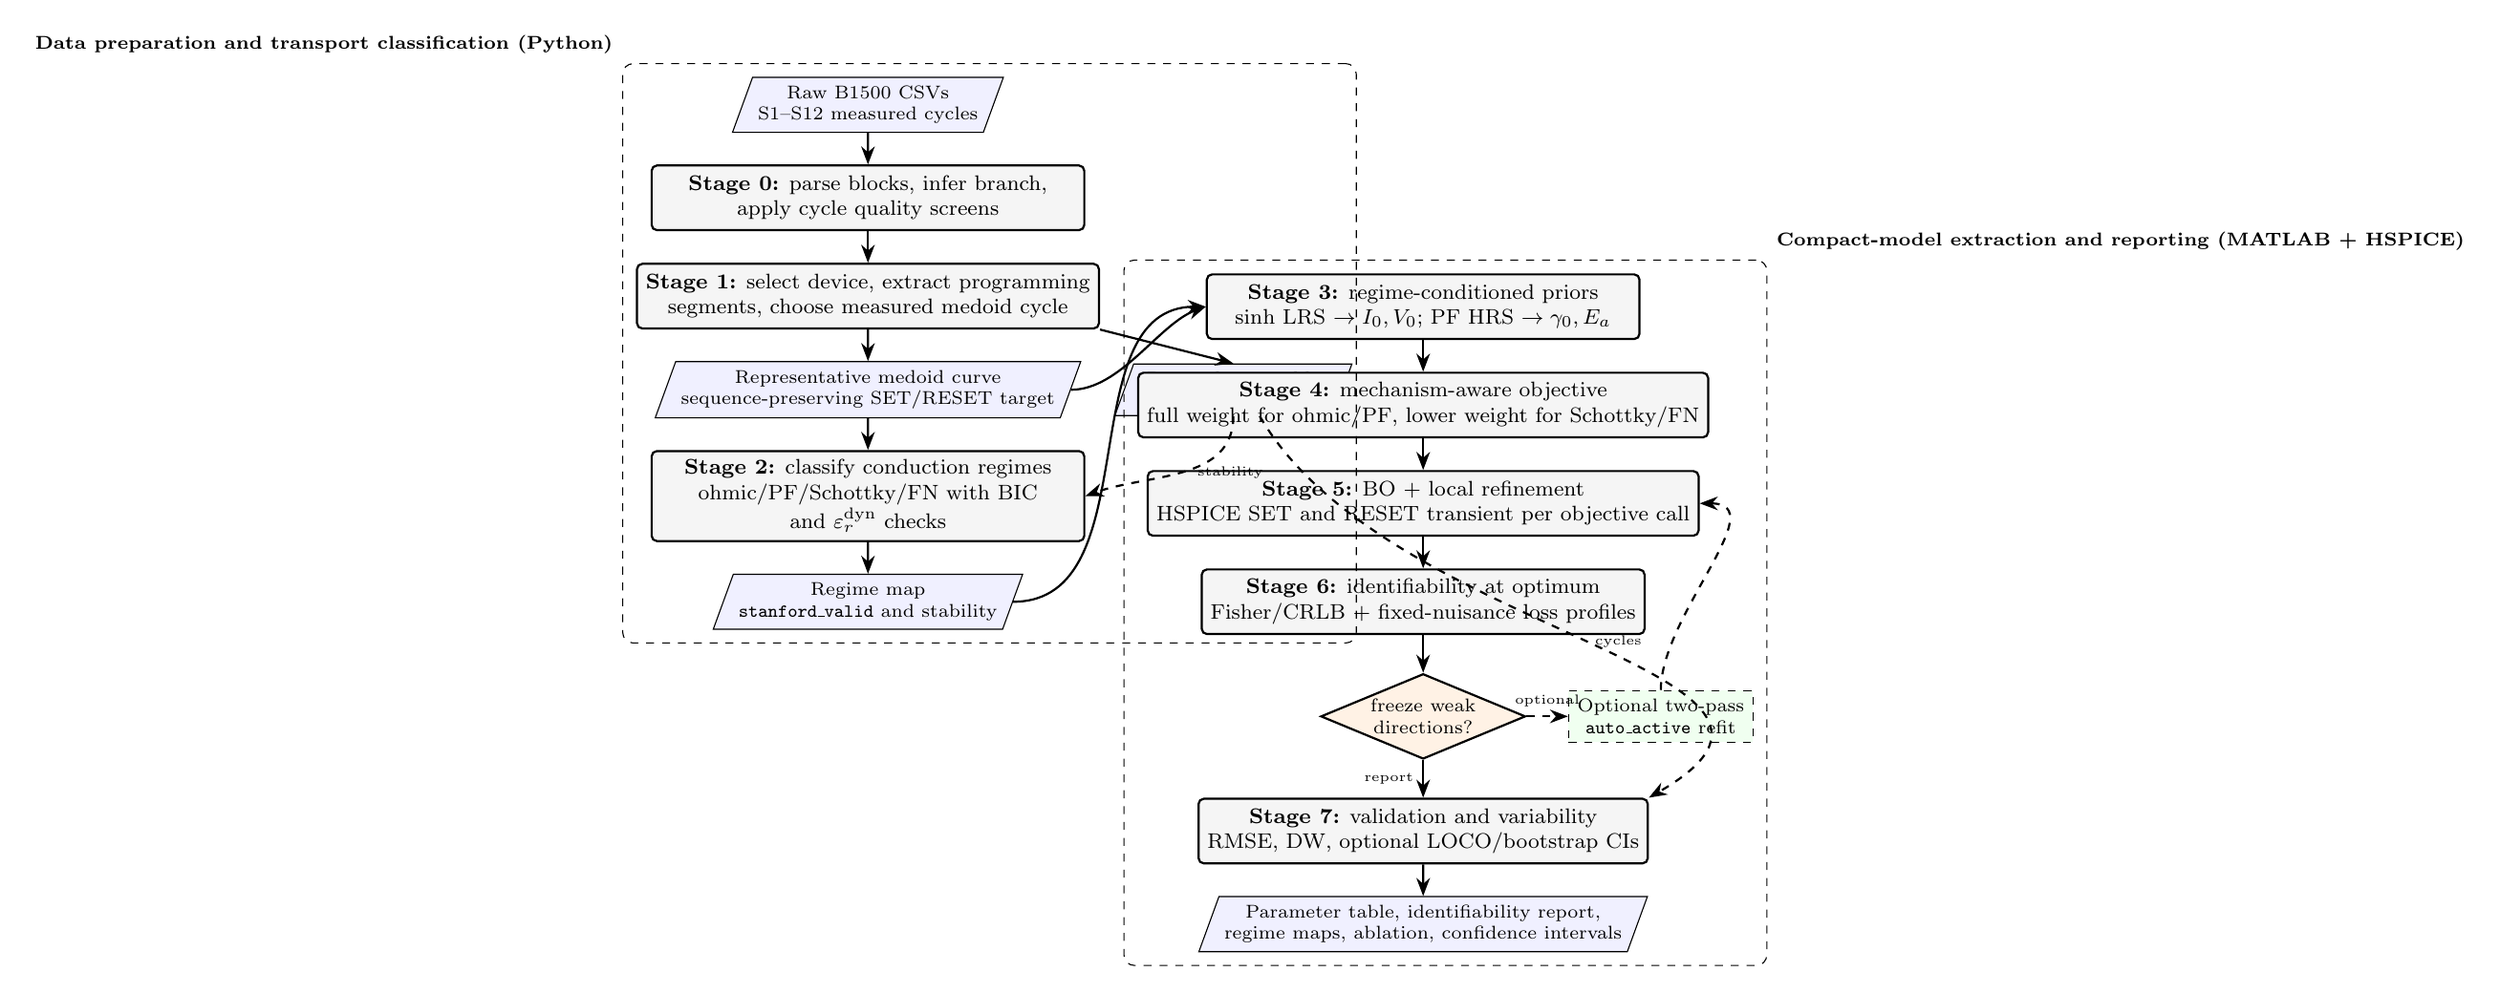
\begin{tikzpicture}[node distance=0.42cm and 0.9cm]

\node[datafile] (raw) {Raw B1500 CSVs\\S1--S12 measured cycles};
\node[stage, below=of raw] (s0) {\textbf{Stage 0:} parse blocks, infer branch,\\apply cycle quality screens};
\node[stage, below=of s0] (s1) {\textbf{Stage 1:} select device, extract programming\\segments, choose measured medoid cycle};
\node[datafile, below=of s1] (rep) {Representative medoid curve\\sequence-preserving SET/RESET target};
\node[datafile, right=0.7cm of rep] (ens) {Per-cycle ensemble\\same selected device};
\node[stage, below=of rep] (s2) {\textbf{Stage 2:} classify conduction regimes\\ohmic/PF/Schottky/FN with BIC\\and $\varepsilon_r^{\mathrm{dyn}}$ checks};
\node[datafile, below=of s2] (rmap) {Regime map\\\texttt{stanford\_valid} and stability};

\node[stage, right=1.6cm of s2.north east, anchor=north west, yshift=2.35cm] (s3) {\textbf{Stage 3:} regime-conditioned priors\\sinh LRS $\to I_0,V_0$; PF HRS $\to \gamma_0,E_a$};
\node[stage, below=of s3] (s4) {\textbf{Stage 4:} mechanism-aware objective\\full weight for ohmic/PF, lower weight for Schottky/FN};
\node[stage, below=of s4] (s5) {\textbf{Stage 5:} BO + local refinement\\HSPICE SET and RESET transient per objective call};
\node[stage, below=of s5] (s6) {\textbf{Stage 6:} identifiability at optimum\\Fisher/CRLB + fixed-nuisance loss profiles};
\node[decision, below=0.5cm of s6] (dec) {freeze weak\\directions?};
\node[stage, below=0.5cm of dec] (s7) {\textbf{Stage 7:} validation and variability\\RMSE, DW, optional LOCO/bootstrap CIs};
\node[sideout, right=0.55cm of dec] (freeze) {Optional two-pass\\\texttt{auto\_active} refit};
\node[datafile, below=of s7] (out) {Parameter table, identifiability report,\\regime maps, ablation, confidence intervals};

\draw[arrow] (raw) -- (s0);
\draw[arrow] (s0) -- (s1);
\draw[arrow] (s1) -- (rep);
\draw[arrow] (s1.south east) -- (ens.north);
\draw[arrow] (rep) -- (s2);
\draw[dasharrow] (ens.south) to[out=-90,in=20] node[right,font=\tiny,xshift=2pt]{stability} (s2.east);
\draw[arrow] (s2) -- (rmap);
\draw[arrow] (rmap.east) to[out=0,in=180] (s3.west);
\draw[arrow] (rep.east) to[out=0,in=200, looseness=0.8] (s3.west);
\draw[arrow] (s3) -- (s4);
\draw[arrow] (s4) -- (s5);
\draw[arrow] (s5) -- (s6);
\draw[arrow] (s6) -- (dec);
\draw[arrow] (dec) -- node[left,font=\tiny]{report} (s7);
\draw[dasharrow] (dec.east) -- node[above,font=\tiny]{optional} (freeze.west);
\draw[dasharrow] (freeze.north) to[out=90,in=0] (s5.east);
\draw[dasharrow] (ens.south east) to[out=-60,in=30, looseness=1.2] node[right,font=\tiny]{cycles} (s7.north east);
\draw[arrow] (s7) -- (out);

\node[draw, dashed, rounded corners, inner sep=5pt, fit=(raw)(s0)(s1)(rep)(ens)(s2)(rmap),
  label={[font=\scriptsize\bfseries]north west:Data preparation and transport classification (Python)}] {};
\node[draw, dashed, rounded corners, inner sep=5pt, fit=(s3)(s4)(s5)(s6)(dec)(s7)(freeze)(out),
  label={[font=\scriptsize\bfseries]north east:Compact-model extraction and reporting (MATLAB + HSPICE)}] {};
\end{tikzpicture}
}%
\caption{End-to-end extraction workflow implemented in the repository.  The
regime map is the connection between the experimental conduction analysis and
the compact-model fit: it selects prior windows, sets mechanism-aware weights,
and helps interpret which parameters can be extracted from the data.}
\label{fig:flowchart}
\end{figure*}

% -------------------------------------------------------------------------
\subsection{Threats to Validity and Reviewer-Facing Limitations}
\label{sec:limitations}

The method makes the following limitations explicit.  First, the released
Stanford current law in Eq.~(\ref{eq:stanford-current}) does not include
separate Schottky or Fowler--Nordheim branches.  The proposed weighting
therefore reduces the influence of such windows on the fitted Stanford
parameters, but it does not make the Stanford model physically complete in
those regimes.  Residual structure in Schottky/FN-dominated windows should be
reported as model mismatch, not hidden.

Second, PF/Schottky discrimination depends on the admissible
$\varepsilon_r^{\mathrm{dyn}}$ bracket.  The bracket $[1,60]$ is deliberately
broad, and the fitted $\varepsilon_r^{\mathrm{dyn}}$ is written to the regime
map so assignments can be audited or sensitivity-tested.

Third, the transient replay is a quasi-static numerical mapping, not the
literal measurement sweep rate.  Parameters such as $\nu_0$ and $E_a$ can
therefore absorb effective time-scale assumptions.  They should be compared
within this protocol and across similarly processed conditions, not treated as
protocol-independent kinetic constants.

Fourth, the reset-side \texttt{gamma0} path is affected by the Verilog-A
negative-bias override in Eq.~(\ref{eq:gamma}).  The branch-split simulation
allows the reset branch to fit through other reset-side parameters, but it
does not remove this structural asymmetry of the released model.

Fifth, the profile-likelihood stage is a fixed-nuisance one-dimensional scan.
It is useful practical evidence of flat directions, but it is not a full
profile with nuisance-parameter reoptimization.  Higher-dimensional sloppy
manifolds are therefore assessed through the Fisher eigenspectrum and the
bootstrap rather than claimed to be fully resolved by the one-dimensional
profiles.

Finally, bootstrap confidence intervals are cluster intervals over cycles of
the selected representative device.  They quantify cycle-to-cycle variability
for that device and fitting protocol.  They do not replace a separate
device-to-device variability study.

% =========================================================================
\begin{thebibliography}{9}\footnotesize

\bibitem{guan2012spice}
X.~Guan, S.~Yu, and H.-S.~P. Wong, ``A SPICE compact model of metal oxide
resistive switching memory with variations,'' \emph{IEEE Electron Device
Lett.}, vol.~33, no.~10, pp. 1405--1407, Oct. 2012.

\bibitem{jiang2014stanford}
Z.~Jiang \emph{et~al.}, ``A compact model for metal--oxide resistive random
access memory with experiment verification,'' \emph{IEEE Trans. Electron
Devices}, vol.~63, no.~5, pp. 1884--1892, May 2016.

\bibitem{chowdhury2025mwscas}
M.~T.~R. Chowdhury, A.~Moazzeni, and G.~Tutuncuoglu, ``Atomic-scale insights
into the switching mechanisms of RRAM devices,'' in \emph{Proc. IEEE 68th
Int. Midwest Symp. Circuits Syst. (MWSCAS)}, Lansing, MI, USA, 2025,
pp. 518--522.

\bibitem{moazzeni2023}
A.~Moazzeni, M.~T.~R. Chowdhury, and G.~Tutuncuoglu, ``The impact of operation
conditions on potentiation, depression and endurance dynamics of tantalum
oxide RRAMs,'' in \emph{Proc. IEEE Int. Integr. Rel. Workshop (IIRW)}, 2023.

\bibitem{chiu2014}
F.-C. Chiu, ``A review on conduction mechanisms in dielectric films,''
\emph{Adv. Mater. Sci. Eng.}, vol. 2014, Art. no. 578168, 2014.

\bibitem{raue2009}
A.~Raue \emph{et~al.}, ``Structural and practical identifiability analysis of
partially observed dynamical models by exploiting the profile likelihood,''
\emph{Bioinformatics}, vol.~25, no.~15, pp. 1923--1929, 2009.

\end{thebibliography}

\end{document}
